\documentclass[a4paper,11pt]{article}

\usepackage[italian]{babel}

\usepackage[latin1]{inputenc}

\usepackage[T1]{fontenc}

\usepackage{graphicx}

\usepackage{indentfirst}

\usepackage{amsmath,amssymb}

\usepackage{enumitem} 

\newcommand{\virgolette}[1]{``#1''}

\usepackage[margin=1in]{geometry} %Smaller margins

\usepackage{lmodern} %Vector PDF

\usepackage{siunitx}

\usepackage{xcolor}

\usepackage{colortbl}

\usepackage{multirow}

\usepackage{rotating}

\usepackage{booktabs}

\usepackage{longtable}

\newcommand*\chem[1]{\ensuremath{\mathrm{#1}}}

\begin{document}

\begin{titlepage}
	\centering
	{\scshape\LARGE Laboratorio di Ottica, Elettronica e \\ Fisica Moderna \par}
	\vspace{1cm}
	{\scshape\Large Relazione di laboratorio 1\par}
	\vspace{1.5cm}
	{\huge\bfseries Spettrometro a reticolo\par}
	\vspace{2cm}

	{\Large\itshape Nicolò Cavalleri, Giacomo Lini e Davide Passaro
	
	(LUN12)}

	\vspace{5cm}
	\vfill
	\begin{abstract}
	
		Di seguito vengono riportate ed esaminate le procedure compiute per la misura della carica dell'elettrone. Sfruttando un supporto fisico che genera un campo elettrico è infatti possibile osservare la variazione di moto di alcune goccioline di olio che si sono caricate elettricamente per strofinio. Dalla variazione di questo moto -- in termini di velocità di caduta e risalita a seconda del verso del campo elettrico, è poi possibile dedurre la quantità di carica che si è \virgolette{sedimentata} sulle goccioline, individuando cos\'i dei multipli della carica di un singolo elettrone.
	
	\end{abstract}

	\vfill
	{\large \today\par}

\end{titlepage}

\newpage

\section{Introduzione}

L'elettrone è una particella subatomica fondamentale dotata di carica \textit{q} che per convenzione è assunta essere una carica negativa. Una delle possibili procedure per effettuare una misura del valore assoluto di questa carica consiste nello studio della dinamica d alcune goccioline di un determinato materiale su cui le cariche si sedimentano (nel caso specifico dell'olio) in diverse condizioni. In particolare è possibile osservare delle differenza quando questa dinamica è influenzata dalla sola forza di gravità (oltre che dall'attrito dell'aria), e quando invece è soggetta anche all'azione di un campo elettrico. 

Nello specifico per una gocciolina in caduta libera, per la quale si suppone una forma sferica, vale la relazione:
\begin{equation}\label{eq_caduta_libera}
\frac{4}{3}\pi r^3 (\rho_o -\rho_a) g - 6 \pi \eta r v_0 =0
\end{equation}
dove $r, \rho_o,\rho_a, \eta, v_0$ sono nell'ordine il raggio della gocciolina, la densità dell'olio e dell'aria, il coefficiente di attrito viscoso dell'aria e la velocità limite della goccia in assenza di campo. Generando un campo elettrico $E$ all'interno del sistema la relazione si modifica e la dinamica delle goccie d'olio obbedisce alla seguente equazione:
\begin{equation}\label{eq_dinamica_campo}
\frac{4}{3}\pi r^3 (\rho_o -\rho_a) g - 6 \pi \eta r v + E q =0
\end{equation}
dove $q$ rappresenta la carica che caratterizza la goccia e $v$ è la nuova velocità limite in presenza di campo.

Noti i valori di $g, \rho_o, \rho_a$ la \ref{eq_caduta_libera} consente, al netto della possibilità di osservare la dinamica della goccia per determianre la velocità con cui questa si muove, di determinarne il raggio. Noto quindi $r$ è possibile generare il campo elettrico all'interno del supporto sperimentale (del tipo di quello rappresentato in figura \ref{millikan} e di cui segue descrizione) per ricavare la carica totale sulla gocciolina d'olio\footnote{Chiaramente queste relazioni sono di natura vettoriale, in quanto si ha a che fare con campi, forze e accelerazioni. L'omissione della notazione vettoriale è qui dovuta alla scelta di snellire leggermente la componente matematica della trattazione teorica del problema.}. Questa considerazione deve valere in maniera indipendentemente dall'orientamento del campo, ed è opportuno in tal senso considerare quando necessario il modulo della velocità.

\begin{figure}[htpb]
	\centering
	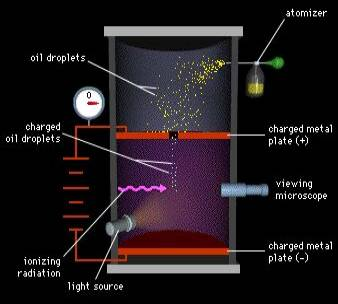
\includegraphics[scale=1]{/../../Immagini/millikan.jpg} 
	\caption{Schema della composizione dell'apparato per la misura della carica dell'elettrone.}\label{millikan}
\end{figure}

Invertendo la \ref{eq_dinamica_campo} è quindi possibile ricavare la carica che caratterizza ognuna delle goccioline su cui è stata effettuata la misura delle velocità. Avendo a che fare con cariche discrete, ci si attende che questi valori siano tutti multipli di un valore \virgolette{unitario} che è proprio la carica del singolo elettrone. Per estrazione di questo termine si pu\'o utilizzare il criterio di massima verosomiglianza stimando il valore di $q$ tramite la ricerca del minimo della parabola individuata dai punti
\[
	S(q)=\sum_{i=0}^{N}\left[\dfrac{Q_i}{k_i(q)}-q\right]^2
\]
dove $Q_i$ rappresenta la carica sulle particelle e $k_i$ è l'intero pi\'u vicino al valore del rapporto $\frac{Q_i}{q}$. Questo valore con il suo errore associato restituisce dunque la miglior stima della carica di un singolo elettrone a partire dai dati ricavati in laboratorio.
\end{document}